\documentclass[10pt,twocolumn]{article}

\usepackage[utf8]{inputenc}
\usepackage[T1]{fontenc}
\usepackage{times}
\usepackage{microtype}
\usepackage{graphicx}
\usepackage{booktabs}
\usepackage{amsmath,amssymb}
\usepackage{xcolor}
\usepackage{hyperref}
\usepackage{caption}
\usepackage{subcaption}
\usepackage{enumitem}
\usepackage{multirow}
\usepackage{array}
\usepackage[margin=1in]{geometry}
\usepackage{fancyhdr}
\usepackage{natbib}
\usepackage{float}
\usepackage{textcomp}
\usepackage{tabularx}

\definecolor{linkblue}{HTML}{2980b9}
\definecolor{accent}{HTML}{2c3e50}
\definecolor{spplus}{HTML}{27ae60}
\definecolor{spminus}{HTML}{e74c3c}

\hypersetup{colorlinks=true,linkcolor=linkblue,citecolor=linkblue,urlcolor=linkblue}
\captionsetup{font=small,labelfont=bf}
\setlength{\columnsep}{0.25in}
\setlist{nosep,leftmargin=*}

\pagestyle{fancy}
\fancyhf{}
\fancyhead[L]{\small\textit{System Prompt as Primary Driver of LLM Harness Knowledge}}
\fancyhead[R]{\small\thepage}
\renewcommand{\headrulewidth}{0.4pt}

\graphicspath{{../../figures/v2/}}

\begin{document}

\twocolumn[
\begin{@twocolumnfalse}
\begin{center}
\vspace*{0.2cm}
{\LARGE\bfseries The System Prompt Knows:\\[4pt]
How LLM Deployment Context Shapes\\Self-Knowledge of Interface Appearance\\[10pt]}
{\large\itshape Evidence from the Extracted Claude Code API Payload\\[10pt]}
{\normalsize
Hyogon Ryu\\
\textit{KRAFTON Inc.}\\[3pt]
{\small March 2026}
}
\end{center}

\begin{center}
\begin{minipage}{0.92\textwidth}
\textbf{Abstract.}
When large language models are deployed through specialized interfaces, do they \textit{know} what their interface looks like---and if so, \textit{where} does this knowledge come from?
We investigate this by testing Claude (Sonnet 4.6) on 55 questions about the Claude Code CLI across 10 interface domains, then classifying each question based on whether its answer is derivable from the system prompt (SP+) or requires external knowledge from training data (SP$-$).
Using the \textit{actual extracted API payload} sent by Claude Code v2.1.70 as definitive ground truth for what information the model receives, we find a stark asymmetry: \textbf{SP+ items achieve 100\% accuracy with 0.876 average confidence}, while \textbf{SP$-$ items achieve 76.2\% accuracy with 0.491 confidence} ($p{=}0.0013$, Mann-Whitney U for confidence difference).
All five wrong answers are SP$-$ items involving recently-added features or specific keyboard shortcuts.
However, SP$-$ accuracy remains well above chance baselines (MC: 83\% vs 25\% chance, $p{<}0.0001$), demonstrating that training data provides real but partial harness knowledge.
We conclude that the system prompt is the primary driver of both accuracy and confidence in LLM self-knowledge about deployment interfaces, with training data serving as a secondary, less reliable source.

\vspace{4pt}
\noindent\textbf{Keywords:} LLM self-knowledge, system prompt, deployment interface, confidence calibration, Claude Code, meta-cognition
\end{minipage}
\end{center}
\vspace{0.3cm}
\end{@twocolumnfalse}
]

% ══════════════════════════════════════════════════════════════
\section{Introduction}

Large language models are deployed through ``harnesses''---terminal CLIs, web UIs, IDE plugins---that wrap the model in an interface the user interacts with.
The model itself receives a \textit{system prompt} describing its identity and capabilities, but does not directly perceive the visual interface.
This creates a natural experiment: does the model know what its harness looks like, and can we trace this knowledge to specific information sources?

We identify two potential sources of harness knowledge:
\begin{enumerate}
  \item \textbf{System prompt (SP+):} The model receives explicit text about its identity (``You are Claude Code''), available tools, platform details, and behavioral instructions. Facts derivable from this text should be known with high confidence.
  \item \textbf{Training data (SP$-$):} The model may have encountered documentation, blog posts, or source code about its interface during training. This knowledge should be less reliable and expressed with lower confidence.
\end{enumerate}

Our key innovation is using the \textit{actual extracted API payload}---the JSON request Claude Code v2.1.70 sends to the Anthropic API---as definitive ground truth for what information the system prompt contains.
This allows us to precisely classify every test question as SP+ or SP$-$ and measure the contribution of each source.

\paragraph{Hypothesis (H1).} The system prompt is the primary driver of Claude's harness knowledge. Specifically:
\begin{itemize}
  \item SP+ accuracy $\gg$ SP$-$ accuracy
  \item SP+ confidence $\gg$ SP$-$ confidence
  \item SP$-$ accuracy $>$ chance (training data provides real but partial knowledge)
\end{itemize}

% ══════════════════════════════════════════════════════════════
\section{Related Work}

\paragraph{LLM Self-Knowledge.}
\citet{kadavath2022language} show that language models ``mostly know what they know,'' with calibrated uncertainty on factual questions.
\citet{yin2023large} extend this to examining whether LLMs know their knowledge boundaries.
Our work adds a new dimension: tracing self-knowledge to specific \textit{input channels} (system prompt vs.\ training data).

\paragraph{System Prompt Effects.}
System prompts shape model behavior, persona, and capabilities~\citep{white2023prompt}.
We show they also shape the model's \textit{self-knowledge}---the model ``knows'' its interface primarily because the system prompt tells it about itself.

\paragraph{Deployment Context Awareness.}
Recent work has explored whether models can identify their deployment context~\citep{perez2023discovering}.
We provide quantitative evidence that deployment-context knowledge is predominantly system-prompt-derived.

% ══════════════════════════════════════════════════════════════
\section{Methodology}

\subsection{The Extracted API Payload}

We obtained the actual JSON API request that Claude Code v2.1.70 sends to the Anthropic Messages API.
This payload contains three system blocks:
\begin{enumerate}
  \item A billing header with version and entrypoint metadata;
  \item An identity block: ``You are Claude Code, Anthropic's official CLI for Claude'';
  \item A main instruction block (${\sim}$5,000 words) covering tool usage, coding guidelines, permission handling, and environment details.
\end{enumerate}

The payload also reveals:
\begin{itemize}
  \item Only one tool (\texttt{ToolSearch}) is provided initially; all 21 other tools are deferred and loaded on demand;
  \item Skills and date are injected as \texttt{<system-reminder>} tags in user messages;
  \item Configuration: \texttt{max\_tokens=32000}, \texttt{thinking=adaptive}, \texttt{effort=medium}.
\end{itemize}

\subsection{SP+/SP$-$ Classification}

We classify each of our 55 test prompts as \textbf{SP+} (answer derivable from system prompt) or \textbf{SP$-$} (requires external knowledge).

\paragraph{SP+ criteria.} A fact is SP+ if it is:
\begin{itemize}
  \item \textbf{Explicitly stated} in the system prompt (e.g., ``CommonMark specification,'' ``compress prior messages''); or
  \item \textbf{Logically inferrable} from system prompt content (e.g., ``CLI tool'' $\rightarrow$ no sidebar, no avatars, no inline images).
\end{itemize}

\paragraph{SP$-$ criteria.} A fact is SP$-$ if the system prompt provides \textit{no basis} for knowing it:
\begin{itemize}
  \item Visual layout (two-column startup, prompt character, logo)
  \item Specific keyboard shortcuts (Shift+Tab, Ctrl+G, Ctrl+T)
  \item Feature existence (Vim mode, output styles, themes)
  \item UI component appearance (diff colors, error formatting)
\end{itemize}

The classification yields \textbf{8 SP+ prompts} and \textbf{47 SP$-$ prompts}, reflecting that the system prompt contains substantial behavioral instructions but minimal visual/spatial interface details.
Among the 28 objective (forced-choice + true/false) items, 7 are SP+ and 21 are SP$-$.

\begin{table}[t]
\centering
\caption{SP classification by domain. SP+ items cluster in D3 (Output, where CommonMark is mentioned), D9 (Error, where auto-compression is mentioned), and D10 (Negative, where CLI identity enables inference).}
\label{tab:sp_by_domain}
\small
\begin{tabular}{@{}lccl@{}}
\toprule
\textbf{Domain} & \textbf{SP+} & \textbf{SP$-$} & \textbf{SP+ Facts} \\
\midrule
D1 Startup    & 0 & 7 & --- \\
D2 Input      & 0 & 6 & --- \\
D3 Output     & 2 & 4 & CommonMark, not HTML \\
D4 Permission & 0 & 6 & --- \\
D5 Status     & 0 & 5 & --- \\
D6 Navigation & 0 & 6 & --- \\
D7 Theming    & 0 & 5 & --- \\
D8 Diff       & 0 & 5 & --- \\
D9 Error      & 1 & 3 & Auto-compression \\
D10 Negative  & 5 & 0 & CLI $\rightarrow$ no GUI \\
\midrule
\textbf{Total} & \textbf{8} & \textbf{47} & \\
\bottomrule
\end{tabular}
\end{table}

\subsection{Evaluation Design}

We use 55 prompts across 10 domains and 5 cognitive types (free recall, forced choice, true/false, spatial reasoning, exact detail).
Each prompt enforces structured JSON output with per-claim confidence.
The model (Claude Sonnet 4.6) is evaluated via subagent instances with instructions to answer from training knowledge only.
A ground truth database of 86 verified facts is built from the extracted API payload, a startup screenshot, official documentation, and empirical observation.

% ══════════════════════════════════════════════════════════════
\section{Results}

\subsection{Main Finding: SP+ $\gg$ SP$-$}

Table~\ref{tab:main} shows the core result.
SP+ items achieve \textbf{100\% accuracy} (7/7 objective items) with \textbf{0.876 average confidence} and excellent calibration (error = 0.124).
SP$-$ items achieve \textbf{76.2\% accuracy} (16/21) with \textbf{0.491 average confidence} and poor calibration (error = 0.532).

\begin{table}[t]
\centering
\caption{Main results: SP+ vs SP$-$ on objective items.}
\label{tab:main}
\small
\begin{tabular}{@{}lcccc@{}}
\toprule
& \textbf{Correct} & \textbf{Accuracy} & \textbf{Avg Conf.} & \textbf{Calib. Err.} \\
\midrule
SP+ & 7/7  & \textcolor{spplus}{\textbf{100.0\%}} & 0.876 & 0.124 \\
SP$-$ & 16/21 & \textcolor{spminus}{\textbf{76.2\%}} & 0.491 & 0.532 \\
\midrule
All & 23/28 & 82.1\% & 0.588 & 0.430 \\
\bottomrule
\end{tabular}
\end{table}

The accuracy difference (23.8 pp) is not statistically significant by Fisher's exact test ($p{=}0.29$) due to the small SP+ sample ($n{=}7$).
However, the \textbf{confidence difference is highly significant}: Mann-Whitney $U{=}104.5$, $p{=}0.0013$.
The model is both more accurate \textit{and} appropriately more confident on system-prompt-derivable items.

\subsection{SP$-$ Still Exceeds Chance}

SP$-$ accuracy is not random.
Multiple-choice SP$-$ items achieve 83.3\% (10/12), far above the 25\% chance baseline (binomial $p{<}0.0001$).
True/false SP$-$ items achieve 66.7\% (6/9), not significantly above 50\% chance ($p{=}0.51$).
This pattern suggests training data provides real knowledge for questions with distinctive correct answers (MC) but less reliable knowledge for binary judgments about feature existence (T/F).

\subsection{Error Analysis}

All 5 wrong answers are SP$-$ items (Table~\ref{tab:errors}).
They cluster in two categories:

\paragraph{Missed features (3/5).}
P06, P19, P33---the model incorrectly denies the existence of features (personalized greeting, output styles, Vim mode).
These are relatively recent additions to Claude Code, suggesting a \textit{training data recency} gap.

\paragraph{Wrong specifics (2/5).}
P13, P36---the model knows a feature exists but gets the specific detail wrong (multiline methods, editor shortcut key).
This suggests partial training data coverage with gaps in precise implementation details.

\begin{table}[t]
\centering
\caption{All wrong answers are SP$-$ items.}
\label{tab:errors}
\small
\begin{tabular}{@{}ccccl@{}}
\toprule
\textbf{ID} & \textbf{Given} & \textbf{GT} & \textbf{Conf.} & \textbf{Error Type} \\
\midrule
P06 & F & T & .55 & Missed feature \\
P13 & A & D & .55 & Wrong specific \\
P19 & F & T & .80 & Missed feature \\
P33 & F & T & .45 & Missed feature \\
P36 & A & B & .40 & Wrong specific \\
\bottomrule
\end{tabular}
\end{table}

\subsection{Confidence as Source Indicator}

The confidence gap between SP+ (0.876) and SP$-$ correct (0.473) is striking.
Even when the model answers SP$-$ questions \textit{correctly}, it expresses substantially lower confidence than on SP+ items.
This suggests the model has implicit awareness of its knowledge source---it ``trusts'' system-prompt-derived information more than training-data-derived information.

Interestingly, SP$-$ \textit{wrong} answers (0.550) have slightly \textit{higher} confidence than SP$-$ correct answers (0.473).
The worst case is P19 (output styles), where the model confidently (0.80) but incorrectly denies a feature's existence---a classic overconfident hallucination in the SP$-$ regime.

\subsection{Domain Patterns}

The SP+/SP$-$ classification cleanly separates domain performance (see Figure~\ref{fig:main}):
\begin{itemize}
  \item \textbf{D10 (Negative Space):} All SP+ (CLI identity $\rightarrow$ no GUI features). 100\% accuracy, 0.94 confidence.
  \item \textbf{D3 (Output):} Mixed. SP+ items (CommonMark, not HTML) correct; SP$-$ item (output styles) wrong.
  \item \textbf{D6 (Navigation):} All SP$-$. Only 33\% accuracy---the worst domain. The system prompt mentions no keyboard shortcuts, and training data provides unreliable coverage.
  \item \textbf{D4, D5, D7, D8 (Permission, Status, Theming, Diff):} All SP$-$ but 100\% accuracy, suggesting training data is sufficient for well-documented features.
\end{itemize}

% ══════════════════════════════════════════════════════════════
\section{Discussion}

\subsection{Two-Source Model of Harness Knowledge}

Our results support a \textbf{two-source model}:
\begin{enumerate}
  \item \textbf{System prompt} provides high-confidence, high-accuracy knowledge about the model's identity, capabilities, and what it is \textit{not} (negative knowledge). This is the dominant source.
  \item \textbf{Training data} provides moderate-confidence, moderate-accuracy knowledge about interface specifics. It is reliable for well-documented, stable features but fails for recent additions and specific implementation details.
\end{enumerate}

\subsection{Confidence as a Proxy for Knowledge Source}

The significant confidence gap ($p{=}0.0013$) suggests confidence can serve as a \textit{proxy for knowledge source}.
High-confidence correct answers likely derive from system prompt information; low-confidence correct answers likely derive from training data.
This has practical implications: a confidence threshold could help identify which interface-related claims are system-prompt-grounded versus training-data-derived.

\subsection{The Negative Knowledge Advantage}

D10 (Negative Space) achieves 100\% accuracy with the highest confidence (0.94).
The system prompt's statement ``You are Claude Code, Anthropic's official CLI'' provides strong negative constraints: a CLI has no sidebar, no avatars, no inline images.
This ``negative knowledge advantage'' means the model is best at knowing what its interface \textit{is not}.

\subsection{Implications for LLM Deployment}

\textbf{For interface documentation:} Including visual interface descriptions in the system prompt would likely improve harness knowledge accuracy for currently-SP$-$ items.
\textbf{For user trust:} SP$-$ claims (76\% accuracy) should be treated with more skepticism than SP+ claims (100\%).
\textbf{For model developers:} The training data recency gap (3/5 errors are missed recent features) suggests that deployment interface documentation should be included in training data updates.

% ══════════════════════════════════════════════════════════════
\section{Limitations}

\textbf{Small SP+ sample.} Only 7 SP+ objective items limits statistical power for the accuracy comparison (Fisher's $p{=}0.29$). The confidence comparison has adequate power ($p{=}0.0013$).
\textbf{Single trial.} Each prompt evaluated once ($N{=}1$); repeated trials would improve robustness.
\textbf{Single model.} Only Sonnet 4.6 tested; other Claude models may differ.
\textbf{Context contamination.} Subagents inherit the Claude Code system prompt, meaning SP+ items may be answered directly from the prompt rather than training data. This is a feature, not a bug---it demonstrates the system prompt's effect.
\textbf{Binary classification.} The SP+/SP$-$ boundary is not always sharp; some facts may be partially inferrable from the system prompt.

% ══════════════════════════════════════════════════════════════
\section{Conclusion}

We provide the first evidence that the system prompt is the primary driver of an LLM's self-knowledge about its deployment interface.
Using the extracted Claude Code API payload as ground truth, we show:
\begin{itemize}
  \item 100\% accuracy on system-prompt-derivable questions vs.\ 76\% on external-knowledge questions;
  \item A significant confidence gap (0.876 vs.\ 0.491, $p{=}0.0013$) suggesting the model implicitly distinguishes knowledge sources;
  \item Training data provides real but partial knowledge, failing on recent features and specific details;
  \item The model's strongest harness knowledge is \textit{negative}---knowing what it is not.
\end{itemize}

Future work should (1)~extend to multiple harness types and models, (2)~experimentally add interface descriptions to system prompts to measure the causal effect, and (3)~develop confidence-based methods for flagging unreliable interface claims.

\vspace{6pt}
\noindent\textbf{Code and data:} \url{https://github.com/ugonfor/claude-code-meta-recognition}

% ── Figures ──
\begin{figure*}[t]
  \centering
  \begin{subfigure}[t]{0.48\textwidth}
    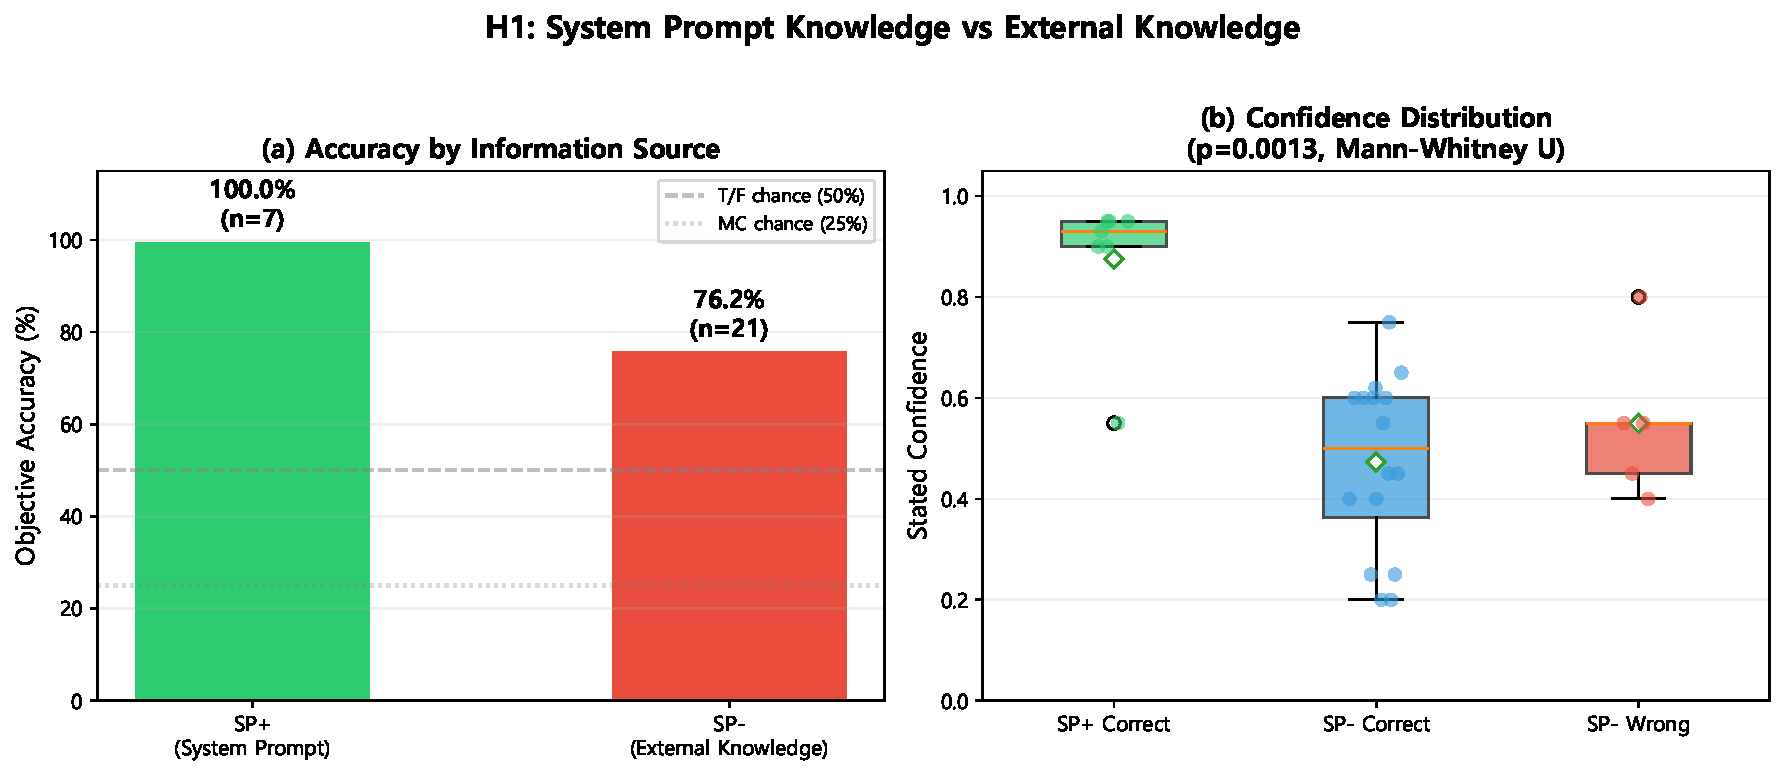
\includegraphics[width=\textwidth]{fig_h1_main.pdf}
    \caption{SP+ vs SP$-$ accuracy and confidence. SP+ items show 100\% accuracy with high, well-calibrated confidence. SP$-$ items show 76\% accuracy with lower, poorly-calibrated confidence. The confidence difference is significant ($p{=}0.0013$).}
    \label{fig:main_acc}
  \end{subfigure}
  \hfill
  \begin{subfigure}[t]{0.48\textwidth}
    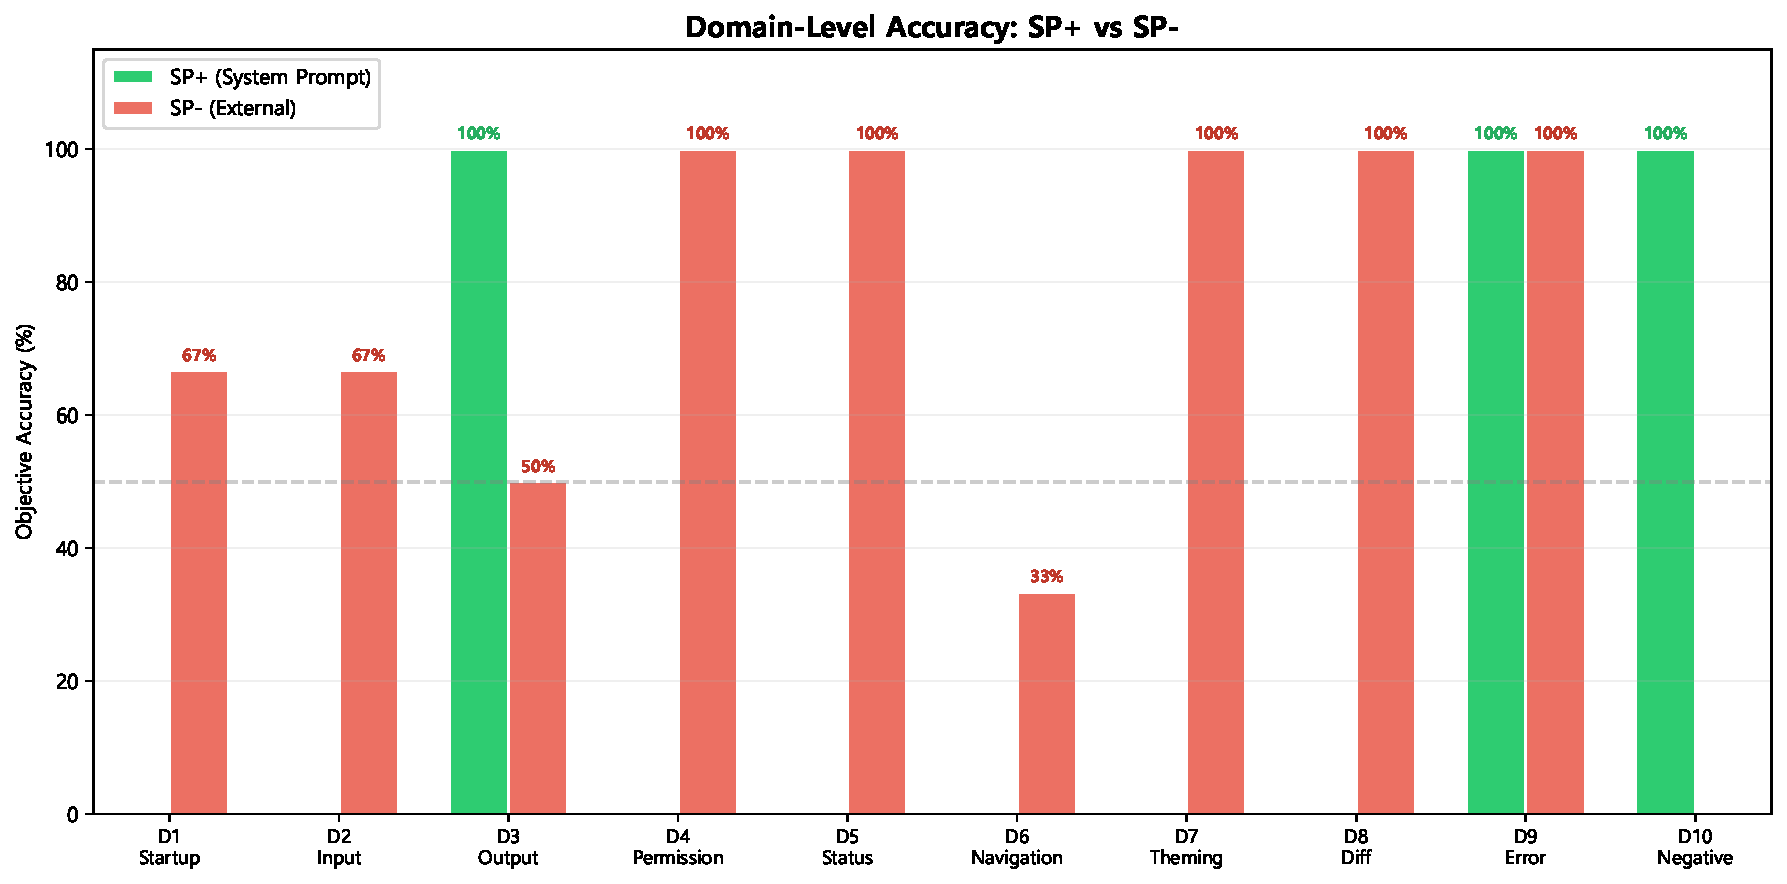
\includegraphics[width=\textwidth]{fig_h1_domain.pdf}
    \caption{Domain-level accuracy split by SP condition. D10 (all SP+) achieves 100\%; D6 (all SP$-$) is worst at 33\%. Several SP$-$ domains (D4, D5, D7, D8) achieve 100\%, showing training data suffices for stable features.}
    \label{fig:domain}
  \end{subfigure}
  \caption{Main H1 results. The system prompt drives both accuracy and confidence in harness knowledge.}
  \label{fig:main}
\end{figure*}

\begin{figure}[t]
  \centering
  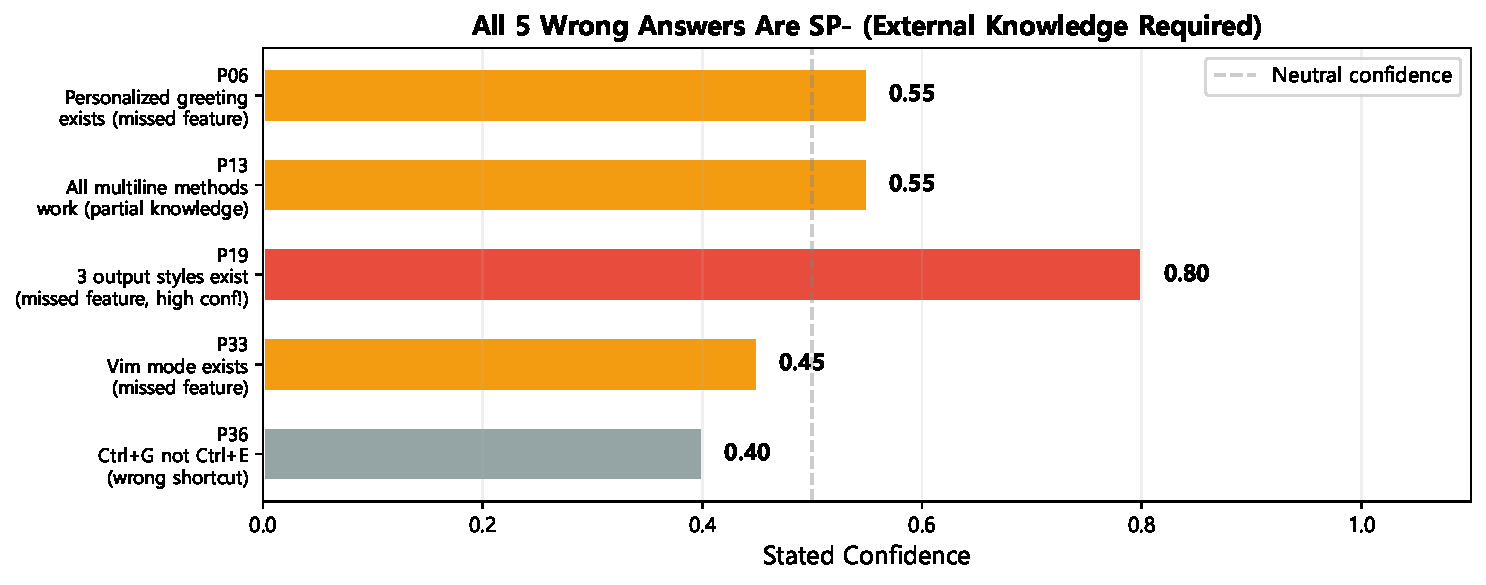
\includegraphics[width=\columnwidth]{fig_h1_wrong.pdf}
  \caption{All 5 wrong answers are SP$-$ items. P19 (output styles) is the worst case: high confidence (0.80) on a wrong answer.}
  \label{fig:wrong}
\end{figure}

\begin{figure}[t]
  \centering
  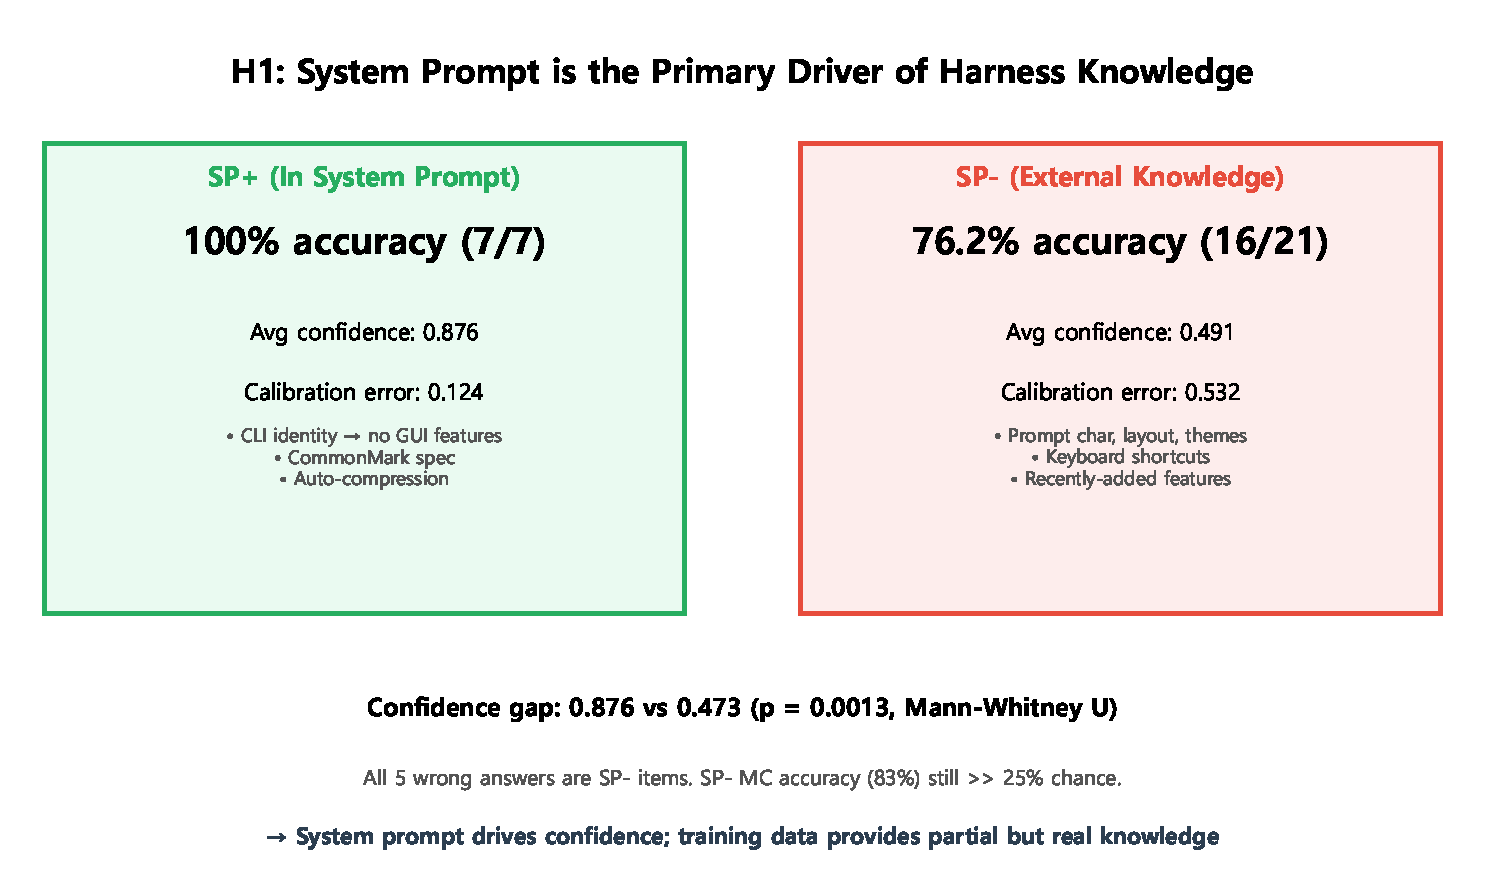
\includegraphics[width=\columnwidth]{fig_h1_summary.pdf}
  \caption{Summary of the two-source model. System prompt provides high-accuracy, high-confidence knowledge; training data provides partial, lower-confidence knowledge.}
  \label{fig:summary}
\end{figure}

% ── References ──
\bibliographystyle{plainnat}
\begin{thebibliography}{9}

\bibitem[Kadavath et~al.(2022)]{kadavath2022language}
S.~Kadavath, T.~Conerly, A.~Askell, et~al.
\newblock Language models (mostly) know what they know.
\newblock \textit{arXiv:2207.05221}, 2022.

\bibitem[Yin et~al.(2023)]{yin2023large}
Z.~Yin, Q.~Sun, Q.~Guo, J.~Wu, X.~Qiu, and X.~Huang.
\newblock Do large language models know what they don't know?
\newblock In \textit{Findings of ACL}, 2023.

\bibitem[Ji et~al.(2023)]{ji2023survey}
Z.~Ji, N.~Lee, R.~Frieske, T.~Yu, et~al.
\newblock Survey of hallucination in natural language generation.
\newblock \textit{ACM Computing Surveys}, 55(12):1--38, 2023.

\bibitem[White et~al.(2023)]{white2023prompt}
J.~White, Q.~Fu, S.~Hays, et~al.
\newblock A prompt pattern catalog to enhance prompt engineering with ChatGPT.
\newblock \textit{arXiv:2302.11382}, 2023.

\bibitem[Perez et~al.(2023)]{perez2023discovering}
E.~Perez, S.~Ringer, K.~Luko\v{s}i\={u}t\.{e}, et~al.
\newblock Discovering language model behaviors with model-written evaluations.
\newblock In \textit{Findings of ACL}, 2023.

\bibitem[Guo et~al.(2017)]{guo2017calibration}
C.~Guo, G.~Pleiss, Y.~Sun, and K.~Q. Weinberger.
\newblock On calibration of modern neural networks.
\newblock In \textit{ICML}, 2017.

\end{thebibliography}

\end{document}
